\documentclass{article}
\usepackage{caption}
\usepackage{subcaption}
\usepackage{amsmath}
\usepackage{amssymb}
\usepackage{mathtools}
\usepackage[margin=0.75in]{geometry}
\usepackage{fancyhdr}
\usepackage{xcolor}
\usepackage{tikz}
\usetikzlibrary{backgrounds}
\usetikzlibrary{calc}
\usepackage[normalem]{ulem} % for strike through text
\setlength{\headheight}{0in}

\newcommand{\problemsep}{\leavevmode\\[0.05in] \rule[\baselineskip/4]{\textwidth}{1pt} \\[0.005in] \rule[\baselineskip]{\textwidth}{1pt}\vspace{-\baselineskip}\leavevmode\\[0.05in]}
\newcommand{\statementsep}{\leavevmode\\[0.005in] \rule[\baselineskip/4]{\textwidth}{0.4pt}\leavevmode\\[0.005in]}
\pagestyle{fancy}
\rhead{\today}
\lhead{Daniel Mortensen}
\chead{Homework 4}

\begin{document}
\noindent\underline{Problem 1}: Please sort all trees on $8$ vertices into homeomorphism classes.
\statementsep
The trees with $8$ vertices are given as \\
\begin{center}
\begin{tabular}{c |c | c | c | c | c | c | c | c |}
 & 1 & 2 & 3 & 4 & 5 & 6 & 7 & 8 \\ \hline
1 & 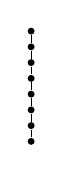
\begin{tikzpicture}[scale=0.05, every node/.style={circle, inner sep=0pt, minimum size=2.5pt, fill=black}, level distance=4cm, level/.style={sibling distance=8cm/#1}]
  \node(root){}
    child {node{}
    child {node{}
	child {node{}
	child {node{}
	child {node{}
	child {node{}
	child {node{}}}}}}}};
\end{tikzpicture} & 
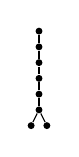
\begin{tikzpicture}[scale=0.05, every node/.style={circle, inner sep=0pt, minimum size=2.5pt, fill=black}, level distance=4cm, level 6/.style={sibling distance=4cm}]
  \node(root){}
    child {node{}
    child {node{}
	child {node{}
	child {node{}
	child {node{}
		child {node{}}
		child {node{}}}}}}};
\end{tikzpicture} &
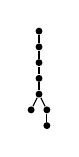
\begin{tikzpicture}[scale=0.05, every node/.style={circle, inner sep=0pt, minimum size=2.5pt, fill=black}, level distance=4cm, level 5/.style={sibling distance=4cm}]
  \node(root){}
    child {node{}
   	child {node{}
	child {node{}
	child {node{}
		child {node{}}
		child {node{}
			child {node{}}}}}}};
\end{tikzpicture} &
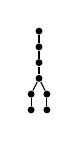
\begin{tikzpicture}[scale=0.05, every node/.style={circle, inner sep=0pt, minimum size=2.5pt, fill=black}, level distance=4cm, level 4/.style={sibling distance=4cm}]
  \node(root){}
    child {node{}
   	child {node{}
	child {node{}
		child {node{}
			child {node{}}}
		child {node{}
			child {node{}}}}}};
\end{tikzpicture} &
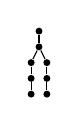
\begin{tikzpicture}[scale=0.05, every node/.style={circle, inner sep=0pt, minimum size=2.5pt, fill=black}, level distance=4cm, level 2/.style={sibling distance=4cm}]
  \node(root){}
    child {node{}
		child {node{}
			child {node{}
				child {node{}}}}
		child {node{}
			child {node{}
				child {node{}}}}};
\end{tikzpicture} &
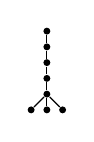
\begin{tikzpicture}[scale=0.05, every node/.style={circle, inner sep=0pt, minimum size=2.5pt, fill=black}, level distance=4cm, level/.style={sibling distance=4cm}]
  \node(root){}
    child {node{}
	child {node{}
	child {node{}
	child {node{}
		child {node{}}
		child {node{}}
		child {node{}}}}}};
\end{tikzpicture} &
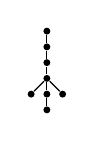
\begin{tikzpicture}[scale=0.05, every node/.style={circle, inner sep=0pt, minimum size=2.5pt, fill=black}, level distance=4cm, level 4/.style={sibling distance=4cm}]
  \node(root){}
    child {node{}
	child {node{}
	child {node{}
		child {node{}}
		child {node{}
			child {node{}}}
		child {node{}}}}};
\end{tikzpicture} &
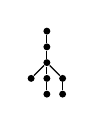
\begin{tikzpicture}[scale=0.05, every node/.style={circle, inner sep=0pt, minimum size=2.5pt, fill=black}, level distance=4cm, level 3/.style={sibling distance=4cm}]
  \node(root){}
    child {node{}
	child {node{}
		child {node{}}
		child {node{}
			child {node{}}}
		child {node{}
			child {node{}}}}};
\end{tikzpicture} \\ \hline
2 & 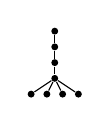
\begin{tikzpicture}[scale=0.05, every node/.style={circle, inner sep=0pt, minimum size=2.5pt, fill=black}, level distance=4cm, level 3/.style={sibling distance=4cm}]
  \node(root){}
    child {node{}
	child {node{}
	child {node{}
		child {node{}}
		child {node{}}
		child {node{}}
		child {node{}}}}};
\end{tikzpicture} &
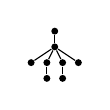
\begin{tikzpicture}[scale=0.05, every node/.style={circle, inner sep=0pt, minimum size=2.5pt, fill=black}, level distance=4cm, level/.style={sibling distance=8cm/#1}]
  \node(root){}
    child {node{}
		child {node{}}
		child {node{}
			child {node{}}}
		child {node{}
			child {node{}}}
		child {node{}}};
\end{tikzpicture} &
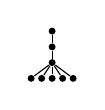
\begin{tikzpicture}[scale=0.05, every node/.style={circle, inner sep=0pt, minimum size=2.5pt, fill=black}, level distance=4cm, level/.style={sibling distance=8cm/#1}]
  \node(root){}
    child {node{}
	child {node{}
		child {node{}}
		child {node{}}
		child {node{}}
		child {node{}}
		child {node{}}}};
\end{tikzpicture} &
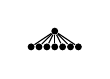
\begin{tikzpicture}[scale=0.05, every node/.style={circle, inner sep=0pt, minimum size=2.5pt, fill=black}, level distance=4cm, level/.style={sibling distance=2cm/#1}]
  \node(root){}
		child {node{}}
		child {node{}}
		child {node{}}
		child {node{}}
		child {node{}}
		child {node{}}
		child {node{}};
\end{tikzpicture} &
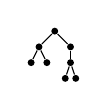
\begin{tikzpicture}[scale=0.05, every node/.style={circle, inner sep=0pt, minimum size=2.5pt, fill=black}, level distance=4cm, level/.style={sibling distance=8cm/#1}]
  \node(root){}
		child {node{}
			child {node{}}
			child {node{}}}
		child {node{}
			child {node{}
				child {node{}}
				child {node{}}}};
\end{tikzpicture} &
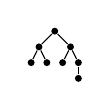
\begin{tikzpicture}[scale=0.05, every node/.style={circle, inner sep=0pt, minimum size=2.5pt, fill=black}, level distance=4cm, level/.style={sibling distance=8cm/#1}]
  \node(root){}
		child {node{}
			child {node{}}
			child {node{}}}
		child {node{}
			child {node{}}
			child {node{}
				child {node{}}}};
\end{tikzpicture} &
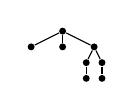
\begin{tikzpicture}[scale=0.05, every node/.style={circle, inner sep=0pt, minimum size=2.5pt, fill=black}, level distance=4cm, level/.style={sibling distance=8cm/#1}]
  \node(root){}
		child {node{}}
		child {node{}}
		child {node{}
			child {node{}
					child {node{}}}
			child {node{}
					child {node{}}}};
\end{tikzpicture} &
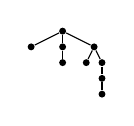
\begin{tikzpicture}[scale=0.05, every node/.style={circle, inner sep=0pt, minimum size=2.5pt, fill=black}, level distance=4cm, level/.style={sibling distance=8cm/#1}]
  \node(root){}
		child {node{}}
		child {node{}
			child {node{}}}
		child {node{}
			child {node{}}
			child {node{}
				child {node{}
					child {node{}}}}};
\end{tikzpicture} \\ \hline
3 & 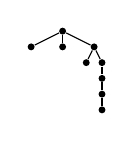
\begin{tikzpicture}[scale=0.05, every node/.style={circle, inner sep=0pt, minimum size=2.5pt, fill=black}, level distance=4cm, level/.style={sibling distance=8cm/#1}]
  \node(root){}
		child {node{}}
		child {node{}}
		child {node{}
			child {node{}}
			child {node{}
				child {node{}
					child {node{}
						child {node{}}}}}};
\end{tikzpicture} &
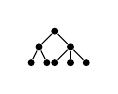
\begin{tikzpicture}[scale=0.05, every node/.style={circle, inner sep=0pt, minimum size=2.5pt, fill=black}, level distance=4cm, level/.style={sibling distance=8cm/#1}]
  \node(root){}
		child {node{}
			child {node{}}
			child {node{}}}
		child {node{}
			child {node{}}
			child {node{}}
			child {node{}}};
\end{tikzpicture} &
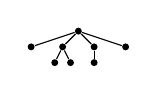
\begin{tikzpicture}[scale=0.05, every node/.style={circle, inner sep=0pt, minimum size=2.5pt, fill=black}, level distance=4cm, level/.style={sibling distance=8cm/#1}]
  \node(root){}
		child {node{}}
		child {node{}
			child{node{}}
			child{node{}}}
		child {node{}
				child {node{}}}
		child {node{}};
\end{tikzpicture} &
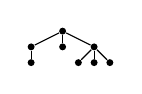
\begin{tikzpicture}[scale=0.05, every node/.style={circle, inner sep=0pt, minimum size=2.5pt, fill=black}, level distance=4cm, level/.style={sibling distance=8cm/#1}]
  \node(root){}
		child {node{}
			child {node{}}}
		child {node{}}
		child {node{}
			child {node{}}
			child {node{}}
			child {node{}}};
\end{tikzpicture} &
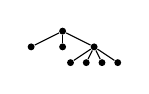
\begin{tikzpicture}[scale=0.05, every node/.style={circle, inner sep=0pt, minimum size=2.5pt, fill=black}, level distance=4cm, level/.style={sibling distance=8cm/#1}]
  \node(root){}
		child {node{}}
		child {node{}}
		child {node{}
			child {node{}}
			child {node{}}
			child {node{}}
			child {node{}}};
\end{tikzpicture} &
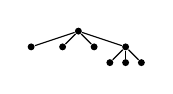
\begin{tikzpicture}[scale=0.05, every node/.style={circle, inner sep=0pt, minimum size=2.5pt, fill=black}, level distance=4cm, level/.style={sibling distance=8cm/#1}]
  \node(root){}
		child {node{}}
		child {node{}}
		child {node{}}
		child {node{}
			child {node{}}
			child {node{}}
			child {node{}}};
\end{tikzpicture}  &
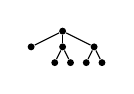
\begin{tikzpicture}[scale=0.05, every node/.style={circle, inner sep=0pt, minimum size=2.5pt, fill=black}, level distance=4cm, level/.style={sibling distance=8cm/#1}]
  \node(root){}
		child {node{}}
		child {node{}
			child {node{}}
			child {node{}}}
		child {node{}
			child {node{}}
			child {node{}}};
\end{tikzpicture} & 
\end{tabular}
\end{center}


and each homeomorphism class is given in the table below along with the index of each corresponding tree. \\
\begin{center}
\begin{tabular}{c | c | c | c}
	Homeomorphism Class & Tree Indices & Homeomorphism Class & Tree Indices \\ \hline
	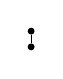
\begin{tikzpicture}[scale=0.05, every node/.style={circle, inner sep=0pt, minimum size=2.5pt, fill=black}, level distance=4cm, level/.style={sibling distance=8cm/#1}]
		\node(root){}
			child {node{}};
	\end{tikzpicture} & (1,1) &
	
\begin{tikzpicture}[scale=0.05, every node/.style={circle, inner sep=0pt, minimum size=2.5pt, fill=black}, level distance=4cm, level/.style={sibling distance=8cm/#1}]
		\node(root){}
			child {node{}
				child {node{}}
				child {node{}}};
	\end{tikzpicture} & (1,2), (1,3), (1,4), (1,5) \\ \hline
		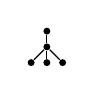
\begin{tikzpicture}[scale=0.05, every node/.style={circle, inner sep=0pt, minimum size=2.5pt, fill=black}, level distance=4cm, level/.style={sibling distance=8cm/#1}]
		\node(root){}
			child {node{}
				child {node{}}
				child {node{}}
				child {node{}}};
	\end{tikzpicture} & (1,6), (1,7), (1,8) &
	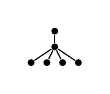
\begin{tikzpicture}[scale=0.05, every node/.style={circle, inner sep=0pt, minimum size=2.5pt, fill=black}, level distance=4cm, level/.style={sibling distance=8cm/#1}]
		\node(root){}
			child {node{}
				child {node{}}
				child {node{}}
				child {node{}}
				child {node{}}};
	\end{tikzpicture} & (2,1), (2,2) \\ \hline
 	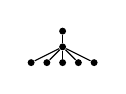
\begin{tikzpicture}[scale=0.05, every node/.style={circle, inner sep=0pt, minimum size=2.5pt, fill=black}, level distance=4cm, level/.style={sibling distance=8cm/#1}]
		\node(root){}
			child {node{}
				child {node{}}
				child {node{}}
				child {node{}}
				child {node{}}
				child {node{}}};
	\end{tikzpicture} & (2,3) &
	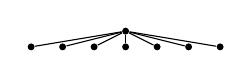
\begin{tikzpicture}[scale=0.05, every node/.style={circle, inner sep=0pt, minimum size=2.5pt, fill=black}, level distance=4cm, level/.style={sibling distance=8cm/#1}]
		\node(root){}
			child {node{}}
			child {node{}}
			child {node{}}
			child {node{}}
			child {node{}}
			child {node{}}
			child {node{}};
	\end{tikzpicture} & (2,4) \\ \hline
	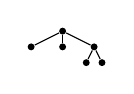
\begin{tikzpicture}[scale=0.05, every node/.style={circle, inner sep=0pt, minimum size=2.5pt, fill=black}, level distance=4cm, level/.style={sibling distance=8cm/#1}]
		\node(root){}
				child {node{}}
				child {node{}}
				child {node{}
					child {node{}}
					child {node{}}};
	\end{tikzpicture} & (2,5), (2,6), (2,7), (2,8), (3,1)&
	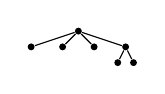
\begin{tikzpicture}[scale=0.05, every node/.style={circle, inner sep=0pt, minimum size=2.5pt, fill=black}, level distance=4cm, level/.style={sibling distance=8cm/#1}]
		\node(root){}
				child {node{}}
				child {node{}}
				child {node{}}
				child {node{}
					child {node{}}
					child {node{}}};
	\end{tikzpicture} & (3,2), (3,3), (3,4) \\ \hline
	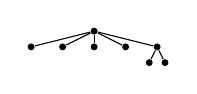
\begin{tikzpicture}[scale=0.05, every node/.style={circle, inner sep=0pt, minimum size=2.5pt, fill=black}, level distance=4cm, level/.style={sibling distance=8cm/#1}]
		\node(root){}
			child {node{}}
			child {node{}}
			child {node{}}
			child {node{}}
			child {node{}
				child {node{}}
				child {node{}}};
	\end{tikzpicture} & (3,5) &
	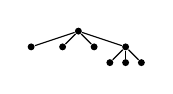
\begin{tikzpicture}[scale=0.05, every node/.style={circle, inner sep=0pt, minimum size=2.5pt, fill=black}, level distance=4cm, level/.style={sibling distance=8cm/#1}]
		\node(root){}
				child {node{}}
				child {node{}}
				child {node{}}
				child {node{}
					child {node{}}
					child {node{}}
					child {node{}}};
	\end{tikzpicture} & (3,6) \\ \hline
	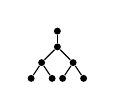
\begin{tikzpicture}[scale=0.05, every node/.style={circle, inner sep=0pt, minimum size=2.5pt, fill=black}, level distance=4cm, level/.style={sibling distance=16cm/#1}]
		\node(root){}
			child {node{}
				child {node{}
					child {node{}}
					child {node{}}}
				child {node{}
					child {node{}}
					child {node{}}}};
	\end{tikzpicture} & (3,7)

\end{tabular}
\end{center}


\problemsep
\noindent\underline{Problem 2}: Show that the graph $G$ (defined later) is not planar in two ways: (1) Use 
Kuratowski's Theorem, and (2) use the Euler identity $n-e+f=2$.
\textsf{Notation:} For $n \in \mathbb{N}$, $[n] = \{1,2,3,\dots, n\}$, and $[0] =\O$.
Define $G = (V,E)$ as follows.  Let $V = \{\mbox{$2$-sets of } [5]\}$, with 
vertices $x$ and $y$ adjacent if and only if $x \cap y = \O$.
\statementsep
\begin{enumerate}
	\item We show that the graph $G$ is not planar with Kuratowski's Theorem which states that a graph is not planar if it contains a subgraph homeomorphic to $K_5$ or $K_{3,3}$. We will show that $G$ contains a subgraph homeomorphic to $K_{3,3}$. Consider the scenario given below and note how the subgraph of $G$ is homeomorphic to $K_{3,3}$ and therefore $G$ is not planar by Kuratowski's Theorem.
		\begin{center}
			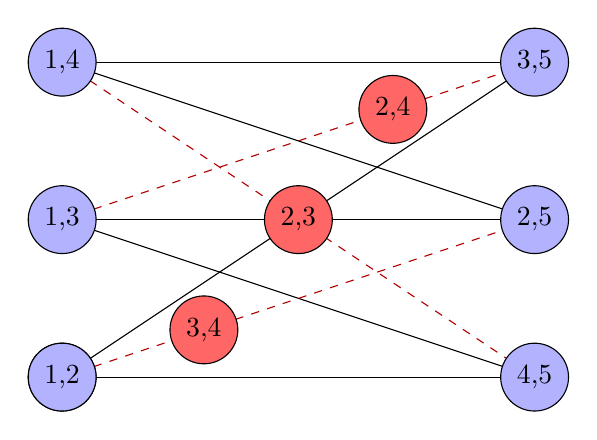
\begin{tikzpicture}[every node/.style={circle, draw=black, fill=blue!30}]
				\node (12) at (0,0){1,2};
				\node (13) at (0,2){1,3};
				\node (14) at (0,4){1,4};
				\node (45) at (6,0){4,5};
				\node (25) at (6,2){2,5};
				\node (35) at (6,4){3,5}; 
				\node[fill=red!60!] (23) at ($(14)!0.5!(45)$) {2,3};
				\node[fill=red!60!] (34) at ($(12)!0.3!(25)$) {3,4};
				\node[fill=red!60!] (24) at ($(13)!0.7!(35)$) {2,4};
				\begin{scope}[on background layer]
					\draw[-] (12.center) -- (35.center);
					\draw[-] (12.center) -- (45.center);
					\draw[-] (13.center) -- (45.center);
					\draw[-] (13.center) -- (25.center);
					\draw[-] (14.center) -- (35.center);
					\draw[-] (14.center) -- (25.center);
					\draw[-] (12.center) node{3,4} (25.center);
					\draw[-, dashed, red!70!black] (14.center) -- (23.center) -- (45.center);
					\draw[-, dashed, red!70!black] (12.center) -- (34.center) -- (25.center);
					\draw[-, dashed, red!70!black] (13.center) -- (24.center) -- (35.center);
				\end{scope}
		\end{tikzpicture}
		\end{center}
	\item We show that the graph $G$ is not planar using Euler's identity ($n - e + f = 2$). In this proof, we will need to prove and use several additional facts:
		\begin{itemize}
			\item {\it Claim:} $G$ has 10 vertices \\
				{\it Proof:} because vertices $x$ annd $y$ are adjacent if and only if $x$ and $y$ are disjoint, then all possible vertices must be all combinations of $[n]$, which is equal to ${n \choose 2}$. Since $n$ in this case is $5$, then we get ${5 \choose 2} = 10$.
			\item {\it Claim: } Every vertex of $G$ has degree 3 \\
				{\it Proof: } Denote an arbitrary vertex in $G$ as $\{a,b\}$ where $a,b \in [5]$. The other elements not in the two-set $\{a,b\}$ are denoted $c,d, \text{and }f$ as there are 5 total elements to choose from. The vertices that contain disjoint sets from $\{a,b\}$ are $\{c,d\}$, $\{c,e\}$, and $\{e,f\}$ so that the degree of $\{a,b\}$ is three..
			\item {\it Claim: } The graph $G$ has 15 edges. \\
				{\it Proof: } We know that $G$ has 10 verticies, each of degree three from the previous two proofs. There will logically be one edge for each degree of a vertex, yielding $10 \times 3$ = 30. However, this counts each edge twice.  Therefore, the total number of edges is $\frac{10\times 3}{2} = 15$.
			\item {\it Claim: } For each pair u,v of nonadjacent vertices in $G$ there exists a unique vertex $w$ that is adjacent to both $u$ and $v$ for all $u\ne v$. \\
				{\it Proof: } Let $u = \{a,b\}$ and $v = \{b,c\}$, where $a,b,c,d,e,f$ are distinct elements in $[5]$. $u$ and $v$ are nonadjacent because they share a value $c$.  We desire to find another vertex $w$ so that $w$ is disjoint from both $u$ and $v$. The elements in $u$ and $v$ are $a,b$ and $c$. Therefore, $u$ and $v$ will both be disjoint from a set comprised of $d$ and $e$. Therefore, $u$ and $v$ will be adjacent to $\{d,e\}$. Therefore, for any arbitrary set of nonadjacent vertices $u$ and $v$ in $G$ there exists uniquely a third point $w$ that is adjacent to both $u$ and $v$.
			\item {\it Claim: } The graph $G$ has no 4-cycle as a subgraph. \\
				{\it Proof: } From the previous proof, let $\{a,b\}$ and $\{b, c\}$ be two nonadjacent vertices in $G$. For there to be a four cycle, there would need to exist two other vertices that were both adjacent to $\{a,b\}$ and $\{b,c\}$, but from the previous proof, we know that there exists a unique point that is adjacent to both $\{a,b\}$ and $\{b,c\}$ so that there cannot be two vertices that are both adjacent to $\{a,b\}$ and $\{b,c\}$. Thus, $G$ cannot have a four-cycle as a subgraph.
			\item {\it Claim: } The graph $G$ has no 4-cycle as a subgraph. \\
				{\it Proof: } Let each element in $[5]$ be denoted $\{a, b, c, d, e\}$ and let $u = \{a,b\}$ and $v = \{c, d\}$ be two adjacent vertices in $G$. If there were to exist a three-cycle in $G$, then there would need to exist a vertex that was adjacent to both $u$ and $v$.  But as there are only $5$ elements to choose from when forming vertices, and 4 of those $5$ are used in $u$ and $v$, then any third vertex must share an element with $u$ or $v$ and thus is not adjacent to both.  Therefore, there cannot exist a three-cycle as a subgraph of $G$.

		\end{itemize}
		With those in mind, we show that $G$ is not planar using Euler's identity. We observe that there is one face for every cyclic subgraph of $G$. We also know that there are no three-cycle or four-cucle subgraphs in $G$. Therefore the cyclic subgraph in $G$ with the smallest degree is a cyclical subgraph of degree 5. The smaller the degree's of the subgraphs, the more faces there are, so by looking at the minimum degrees of faces, we effectively look at the maximum number of faces. Assume without loss of generality that all faces have degree 5.  Then from Lemma 11.2.1 in the lecture notes, we know that
		\begin{equation*}
			\sum_{i = 1}^n d(f_i) = 2e(G).
		\end{equation*}
		which implies that
		\begin{equation*}
			5\sum_{i=1}^n 1 = 2e(G)
		\end{equation*}
		where $n$ is the number of faces. The last equation then implies that the maximum number of faces is equal to $\frac{2e(G)}{5} = \frac{2\times 15}{5} = 6$. If we substitute the values for the number of edges, vertices, and maximum number of faces into euler's identity, then the maximum value that euler's identity can yield is 
		\begin{equation*}
			10 - 15 + 6 = 1.
		\end{equation*}
		Since euler's identity cannot be equal to 2, then $G$ cannot be planar.
\end{enumerate}
\problemsep
\noindent\underline{Problem 3:} Please prove that no pair of the directed graphs in the figure below are 
isomorphic.
\begin{center}
    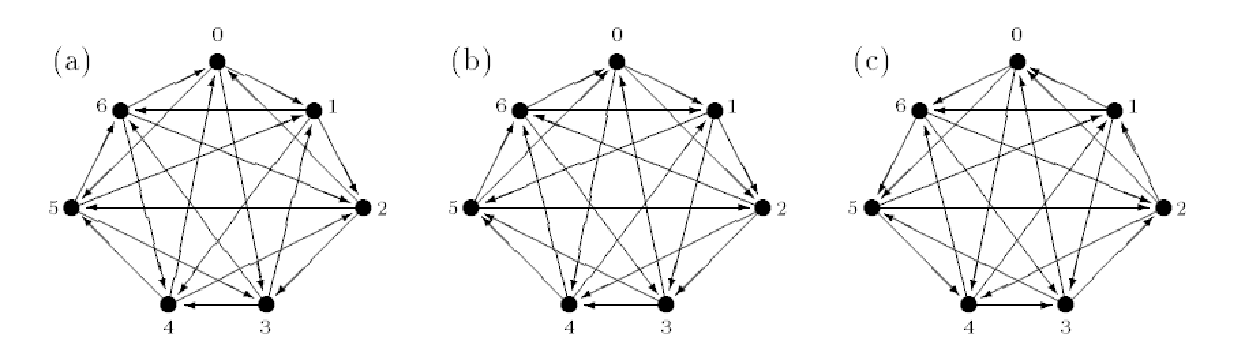
\includegraphics[scale=0.75]{media/reg7Ts.pdf}
\end{center}
\statementsep
The figure below displays the number of 3, 4, 5, 6, and 7 element cyclical subgraphs of $G$. Note how the number of 4, 5, 6, and 7 cycle sub-graphs is different for all three graphs.  This suggests that the structure of each graph is inherently different and consequently that there does not exist an isomorphism between any of the three graphs.
\begin{center}
	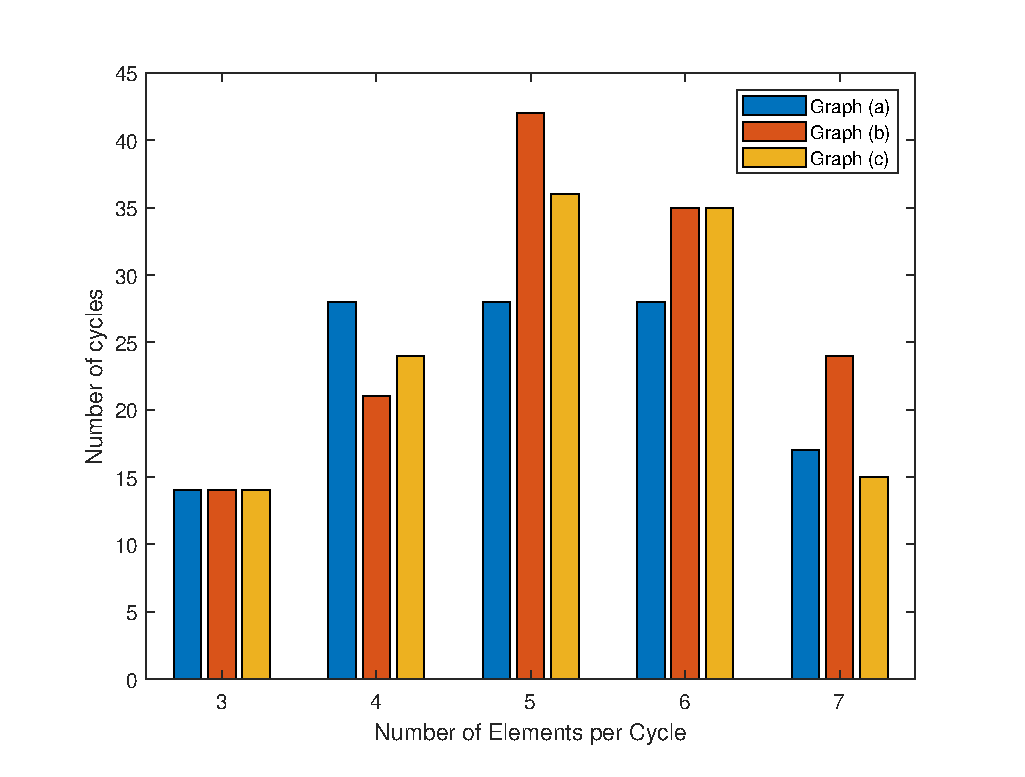
\includegraphics{media/graphComparison.eps}
\end{center}
\end{document}
